\documentclass[12pt,preprint]{aastex}
%\usepackage{thumbpdf}
\usepackage{amssymb,float}
\usepackage{psfig,graphicx} 
\usepackage{fullpage,mathtools}
\usepackage{mathrsfs}
\usepackage{natbib}
\usepackage{color}
\usepackage{bm}
\usepackage[title,titletoc,toc]{appendix}
\bibliographystyle{apj}

\addtolength{\oddsidemargin}{-.5in}
\addtolength{\evensidemargin}{-.5in}
\addtolength{\textwidth}{0.5in}

\title{Detailed User guide for the \\ Simple MCMC Orbit Determination Tool \\(SMODT)}
\author{Kyle Mede}
\date{\today}

\begin{document}

\maketitle

% List contents then list of figures
\tableofcontents


\section{Introduction}

These are the outlines of the functions that act as the models to calculate the orbital elements for either a binary star system or planet orbit.  The equations are the result of combining Kepler's laws, the definitions of the orbital elements and the naturally occurring symmetries and rules of a stable binary system.

There are both Python and C++ versions of these functions/models.  The bulk of the multi-process and file management,  post analysis and plotting of the results is done in Python while the computational stages of the simulation are done in C++ to take advantage of its speed.  A more detailed description of these issues and the simulator will be in another document to be written later.  All three astrometry models described here have been tested and produce the same resulting values/fit to within approximately 10 significant figures, well past the accuracy limits placed on the parameters by their associated 68\% or 95\% errors.

%-----------------------------------------------------------
%\citet{batten}
%\pagebreak
%\bibliography{SMODT-citations}
%\clearpage
%-----------------------------------------------------------
\pagebreak
\subsection{Measured Astrometric Values}\label{sec:MeasAstrometry}

There are multiple ways to visually represent an astrometric system, and thus the measured values must be clearly understood to ensure they are correct before using them as inputs to the SMODT orbital model and plotting routines.

The orientation and definition of x and y depends on the choice of view of the binary system.  The two most common of these are the telescope and the naked eye view, seen in Figure \ref{fig:4} compared to a standard Cartesian coordinate system.  As direct observations of binary systems result in images matching the orientation of the telescope's view, and that in many different situations angles are commonly measured from the positive ``x" axis, the combination of these two led to the standard conventional coordinate system given by a) in Figure \ref{fig:5}; thus, E=y and N=x.  This convention can also be seen used in Figure \ref{fig:apparentTrueEllipses}, showing the geometric meaning of the Thiele-Innes elements along with the apparent and true orbital ellipses of an example binary system.  While that is the conventional coordinate system for measuring astrometric data, when plotting the data along with the predicted orbit more recently people follow that of b) in Figure \ref{fig:5}.  Therefore, as long as the proper coordinate systems are being used the appropriate x and y values can be calculated with the equations (\ref{eq:28-2a} \& \ref{eq:28-2b}).

To help avoid the possible confusion due to the different definitions of x and y, the more easily understood $\phi$ and $\rho$, with associated errors, are used as the input data coordinates.  The models and post-processing plotting routines will then appropriately handle the required conversions.

In the case where the data is measured as the difference in Right Ascension ($\alpha$) and Declination ($\delta$) of the companion from the primary star, in units of [$\arcsec$], these match the E=y and N=x respectively.  This allows for direct comparison of the data to the values calculated in equations  (\ref{eq:28-1a}) and (\ref{eq:28-1b}).  If these units need to be converted to $\phi$ and $\rho$, then the following conversions can be used.

The respective x and y values from the measured position angle ($\phi$) and separation angle ($\rho$) are given by:
\begin{subequations}
\begin{align}\label{eq:28-2a}
x_{TH-I}& = \rho \cos(\phi) = y_{plot} = North = \delta\\
\label{eq:28-2b}
y_{TH-I}& = \rho \sin(\phi) = x_{plot} = East = \alpha
\end{align}
\end{subequations}

with $\phi$ in units of [radians] and $\rho$ in [$\arcsec$].

The error in the data values in the new coordinate system would then be:

\begin{subequations}
\begin{align}\label{eq:28-3a}
\sigma_{x}=\Delta x_{TH-I}& = x_{TH-I} \sqrt{\bigg(\frac{\Delta\rho}{\rho}\bigg)^2 +\bigg(\frac{\cos(\phi+\Delta\phi)-\cos(\phi)}{\cos(\phi)}\bigg)^2} \\
\label{eq:28-3b}
\sigma_{y}=\Delta y_{TH-I}& = y_{TH-I} \sqrt{\bigg(\frac{\Delta\rho}{\rho}\bigg)^2 +\bigg(\frac{\sin(\phi+\Delta\phi)-\sin(\phi)}{\sin(\phi)}\bigg)^2} 
\end{align}
\end{subequations}

If the astrometric values measured are as East and North, both in units of[$\arcsec$], the following equations can be used to convert them to those of $\phi$ and $\rho$: 

\begin{subequations}
\begin{align}\label{eq:22-a}
\rho& = \sqrt{(East)^2+(North)^2} \\
\label{eq:29-b}
\phi& = arctan\bigg(\frac{East}{North} \bigg) 
\end{align}
\end{subequations}

with matching errors:

\begin{subequations}
\begin{align}\label{eq:30-a}
\sigma_{\rho}=\Delta \rho& = \rho \bigg(\frac{|\Delta North \times North| + |\Delta East \times East|}{North^2 + East^2}\bigg)\\
\label{eq:30-b}
\sigma_{\phi}=\Delta \phi& = \Bigg|\frac{East}{North}\Bigg|\frac{\sqrt{\big( \frac{\Delta East}{East} \big)^2+\big(\frac{\Delta North}{North} \big)^2}}{1+\big(\frac{East}{North} \big)^2   } 
\end{align}
\end{subequations}

\begin{figure}[h]
\begin{center}
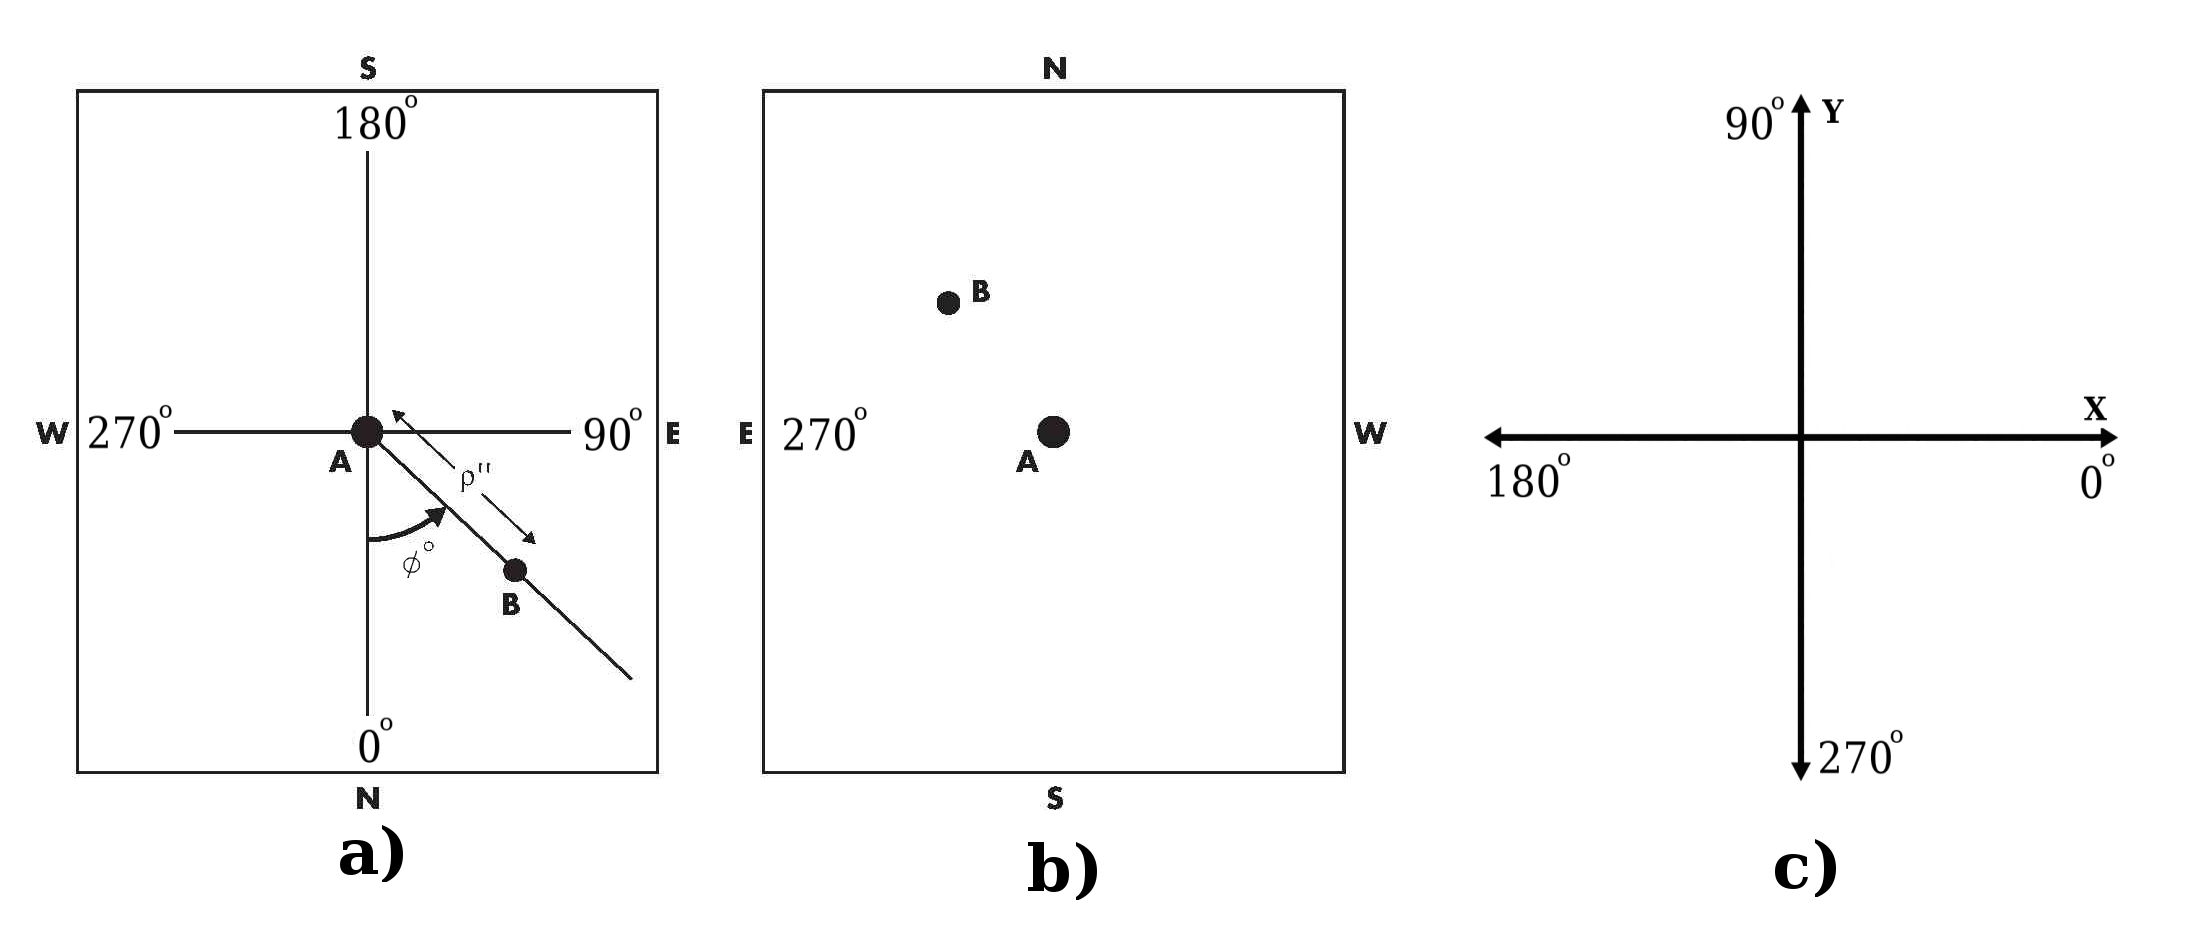
\includegraphics[scale=0.9]{Figures/Argyle-oribit-plots1-cropped-AND-cartesianCoordsPlot.jpg}
\caption[View of a Binary System]{ View of a binary system through a) A telescope, b) The naked eye, compared to c) The Cartesian coordinate system. \citet{Argyle}. }
\label{fig:4}
\end{center}
\end{figure}

\begin{figure}[h]
\begin{center}
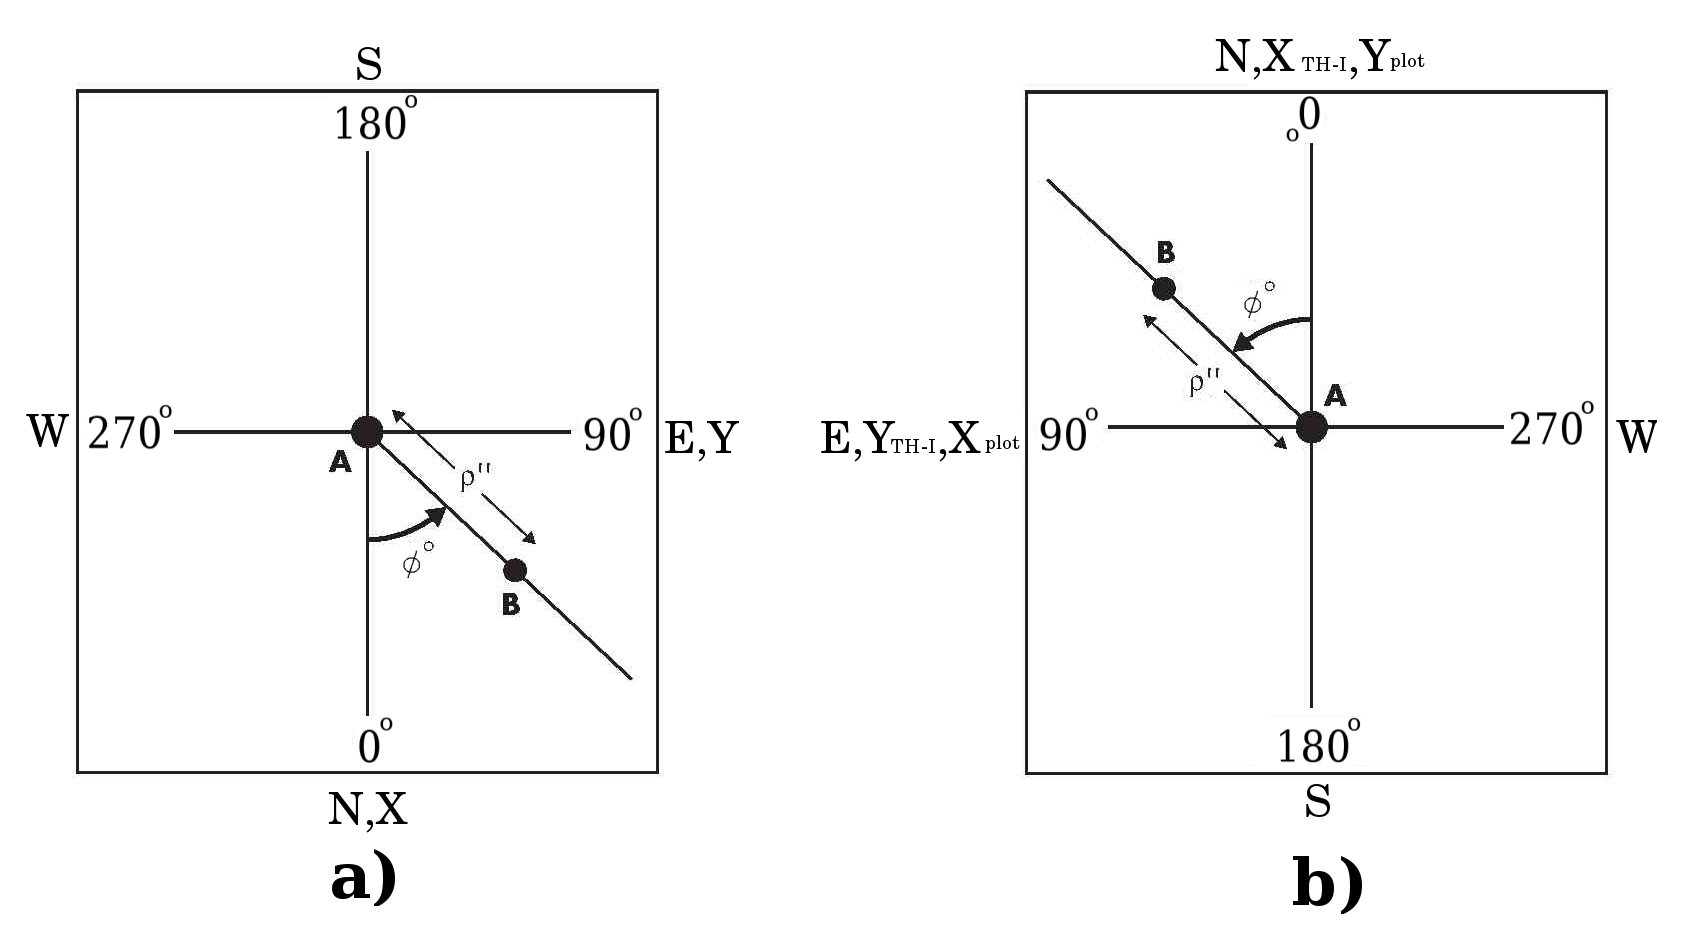
\includegraphics[scale=1.3]{Figures/Argyle-Observation-and-plot-conventions.jpg}
\caption[Measured and Plotted Atrometric data]{ Conventional orientations and coordinates for a) measuring and b) plotting the astrometric values of a binary system. }
\label{fig:5}
\end{center}
\end{figure}

\begin{figure}[h]
\begin{center}
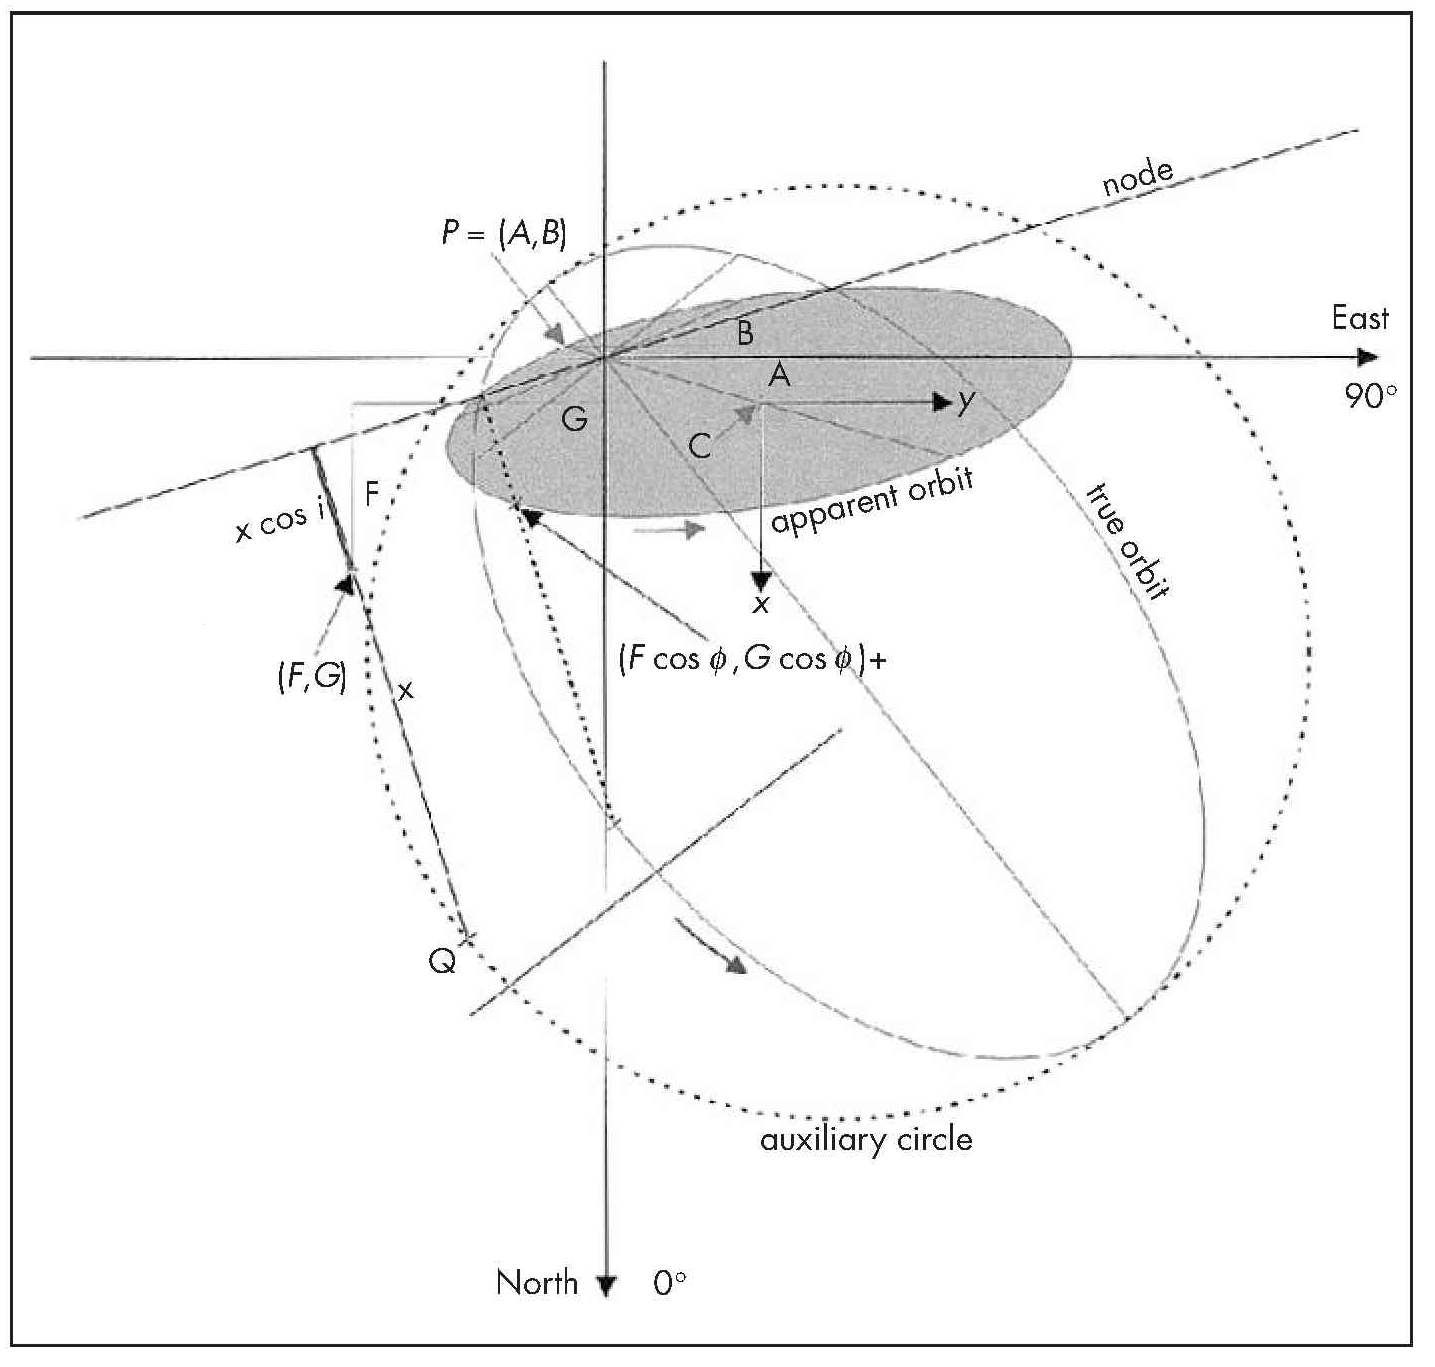
\includegraphics[scale=1.5]{Figures/Argyle-oribit-plots2-cropped2.jpg}
\caption[Apparent and True orbital ellipses]{ Plot of apparent and true orbital ellipses, and the Thiele-Innes elements, \citet{Argyle}. }
\label{fig:apparentTrueEllipses}
\end{center}
\end{figure}


\clearpage

%-----------------------------------------------------
\subsection{Binary Orbital Elements}\label{sec:BinaryOrbElements}

When observing a binary system with either the naked eye, or with a telescope, what can be seen is their positions in the plane of the sky, see Figure \ref{fig:4}.  As was discovered by Johannes Kepler in the early 17$^{th}$ century binary systems will move in elliptical orbits around the center of gravity.  In most cases though, the elliptical path seen, commonly referred to as the `apparent ellipse', will be that orbit projected onto the plane of the sky.  This is because most orbital systems do not orbit perfectly in the plane of the sky and instead lie in the system's `orbital plane'.  So, with a sufficient number of observations over a long enough amount of time, the apparent ellipse can be drawn, but not the true orbital path in the orbital plane.  In order to find the exact shape of the true ellipse and its orientation with respect to the plane of the sky, the 6 parameters called the `orbital elements' must be calculated.

The orbital elements that describe the orientation of the orbital plane to the plane of the sky are the inclination, {\it i}, and the longitude of the ascending node, $\Omega$.  As can be seen in Figure \ref{fig:OPvsSky}, {\it i} is the angle between the the two planes centered on the intersection line.  In the case where the position angles measured are increasing with time, the orbital motion is considered direct, or prograde, and {\it i} will lie in the range 0$^{\circ}$-90$^{\circ}$.  On the other hand, if they decrease with time, the motion is retrograde and it will take values of 90$^{\circ}$-180$^{\circ}$, \citep{heintz}.  The intersecting line between the two planes is known as the `line of nodes' with the ascending node being the point on the orbit passes upward through the plane of the sky, and the descending node being on the other side when the orbit passes through moving downwards.  Most commonly measured in the plane of the sky from North to East, $\Omega$ is the angle to the ascending node, shown as `N' in Figure \ref{fig:orbElements}; due to this, $\Omega$ is sometimes referred to as the position angle of the line of nodes, \citep{binnendijk}.  Unfortunately, just by looking at the system there is no way to tell if the body is truly moving upward at a the ascending node due to the apparent orbit being a projection onto the sky.  To handle the problem temporarily, a convention of $\Omega$ being between 0$^{\circ}$-180$^{\circ}$ is commonly used.  This 180$^{\circ}$ discrepancy can be removed when radial velocity data also exists for the system.  If the orbital motion of the object is directed away from the Earth, shown by positive velocities, that node is confirmed to be the ascending node and the convention holds.  Else, the node is actually the descending node and the location of the ascending node would be within 180$^{\circ}$-360$^{\circ}$, \citep{heintz}.
 
\pagebreak

\begin{figure}[h]
\begin{center}
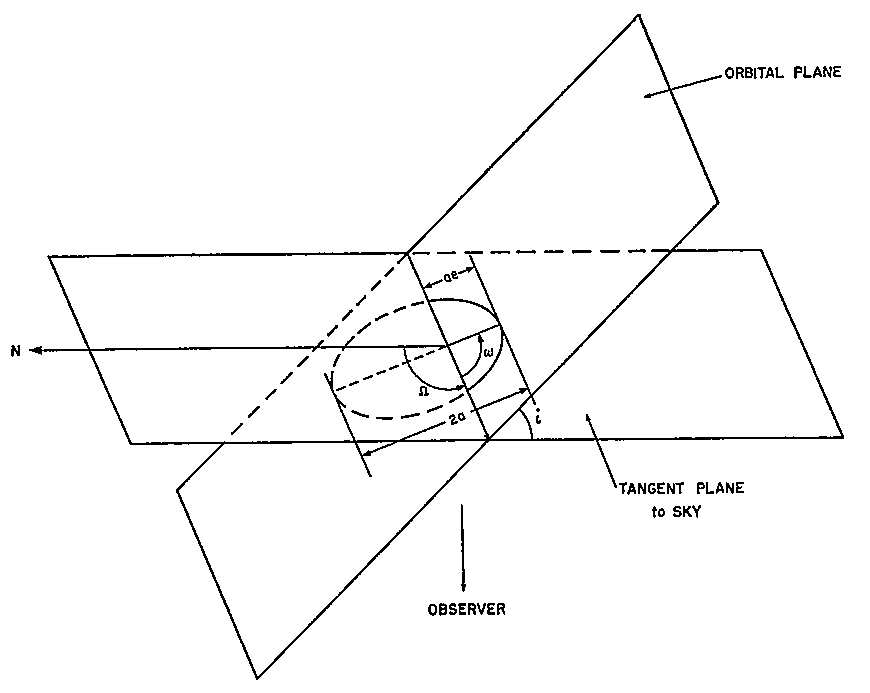
\includegraphics[scale=0.575]{Figures/BattenPG8Fig.jpeg}
\caption[Orbital Plane vs Plane of Sky]{ Orbital plane and the tangent plane to the sky  From \citet{batten}. }
\label{fig:OPvsSky}
\end{center}
\end{figure}

\begin{figure}[h]
\begin{center}
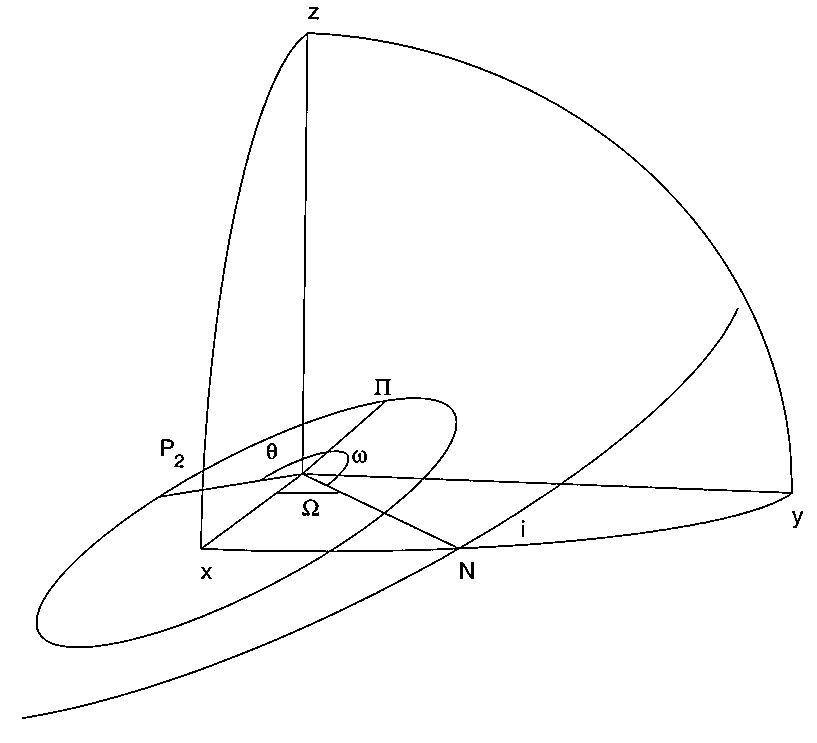
\includegraphics[scale=0.5]{Figures/HilditchPG41Fig.jpeg}
\caption[Orbital Elements]{ The relative orbit of a  binary located in three dimensions to show the orbital elements of its orbit.  From \citet{hilditch}. }
\label{fig:orbElements}
\end{center}
\end{figure}


The two orbital elements that define the shape of the true orbital ellipse are the eccentricity, {\it e}, and the semi-major axis, {\it a}.  Looking at Figure \ref{fig:orbEllipse}, the semi-major axis half the length of the line between the two most distant points on an ellipse.  The two focus points along this line are represented by F and F' with the distance from the center of the ellipse to either of these being simply a{\it e}.  The value of the eccentricity for an ellipse take values of [0,1.0], with the value 0 making it a circle and 1.0 a parabola.  For a binary system, both of the bodies are actually moving with respect to a common center of gravity, see Figure \ref{fig:ellipseComparison}.  A standard convention to simplify this is to put the larger body at a focal point and consider the apparent path of the other body as the combined elliptical orbit.  By doing the math, one can check that this is a valid convention choice assuming  $a= a_1+ a_2$.  


\begin{figure}[h]
\begin{center}
\includegraphics[scale=0.81]{Figures/Ellipse-Modified2.jpeg}
\caption[Orbital Ellipse]{ The ellipse of an orbit in the orbital plane. }
\label{fig:orbEllipse}
\end{center}
\end{figure}

\begin{figure}[h]
\begin{center}
\includegraphics[scale=0.22]{Figures/Ellipse-ModifiedNEW2.jpeg}
\caption[Single vs Dual Orbital Ellipses]{ A comparison of a single combined ellipse to the original individual ellipses for a binary system.}
\label{fig:ellipseComparison}
\end{center}
\end{figure}

The last two orbital elements needed to fully describe an orbit in three dimensional space are the mean anomaly, {\it M}, and the argument of periapsis, $\omega$.  The point of periapsis is where the two bodies are the closest to each other, shown as $\Pi$ in Figures \ref{fig:orbElements} and \ref{fig:orbEllipse}.  $\omega$ is then just the angle between the ascending node and $\Pi$ measured in the orbital plane, \citep{heintz}; sometimes this angle is referred to as the longitude of periapsis to match the naming of the longitude of the ascending node, \citep{hilditch}.  The mean anomaly, {\it M} defines the position of the secondary body through its orbit, but not as a directly measurable value, other parameters are commonly chosen to replace it in the orbital elements.  {\it M} is calculated following equations (\ref{eq:nAndMa} \& \ref{eq:nAndMb}), where {\it n} is the mean motion, {\it t} is the time the system is being observed and {\it T} is the time the second body was at the periapsis point, usually called the time of last periapsis.  The other parameters more commonly used are the period of the orbit and {\it T}.  By using these parameters the semi-major axis is not strictly required if the mass of the two bodies is known, as Kepler's third law of motion can be used to calculated it, shown in Equation (\ref{eq:KepThird}), where $M_1$ and $M_2$ are the masses of the two bodies.


\begin{subequations}
\begin{align}\label{eq:nAndMa}
n &= \frac{2\pi}{P} \\
\label{eq:nAndMb}
M &= n \bigg( \frac{(t-T)}{365.25} \bigg)
\end{align}
\end{subequations}

\begin{equation}\label{eq:KepThird}
P^2 = \bigg[\frac{4\pi^2a^3}{G(M_1+M_2)} \bigg]
\end{equation}

Therefore, either [{\it i}, $\Omega$, {\it e}, {\it a}, $\omega$, {\it M}] or [{\it i}, $\Omega$, {\it e}, $\omega$, {\it P}, {\it T}] can be used to fully describe any binary orbit in space.  Later in Section \ref{sec:models} some of the orbital models for converting between the observed apparent ellipse and the true ellipse will be described. 

\clearpage
%----------------------------------------------------------------------------------------------------------
\section{Simulator Data Modes}\label{sec:simDataModes}

There are 3 main modes that SMODT can be ran in (Astrometry only, Radial Velocity only, or 3D).  Each of these have been tested, but there are important things to keep in mind when using any of them.
%----------------------
\subsection{Astrometry only (DIonly)}
%When astrometry measurments were first used to fit the orbits of companion planets or stars, the companion was commonly not seen and only the movement of the primary with respect to the background stars was measured.  As was discussed in section (\ref{sec:BinaryOrbElements}), it is possible to fit to the the orbits of the primary, secondary or the combined orbit.  Recently, the measured astrometry is for the secondary with respect to the primary, and therefore it is the combined orbit that is of interest.  In the combined orbit, all the orbital elements are the same, except the semi-major axis ($a$) and the argument of periapsis ($\omega$).  To allow the user to fit to whateever orbit they like, a number of special settings are provided.
Most of the key differences for fitting choices are in the Radial Velocity model.  In some cases there is a need to add a fixed 180$^{\circ}$ to the $\omega$ value used in the Astrometry model.  Thus, the following parameter is available to do that:

{\bf argPeriPlusDI}\\
This is a fixed value in degrees to be added to the value of the $\omega$ used in the DI model. ie. $\omega_{DImodel}=\omega+argPeriPlusRV$.
%----------------------
\subsection{Radial Velocity only (RVonly)}
The key reason for needing to fit to different Radial Velocity orbits, is the occasional lack of clarification of what the provided RV data is of and which orbit is being fit.  In all cases it is only the values of $a$ and $\omega$ that differ.  Please keep in mind that instead of calculating the semi-major amplitude ($K$) from $a$, $i$, $P$ and $e$, one can set the max and min values allowed for the Inclination to zero and thus vary $K$ directly.  Also, the value of $\omega$ for the primary and secondary are offset from eachother by +/-180$^{\circ}$, with the sign being irrelivant as they both cause the resulting velocities to be of the opposite sign (ie. if primary velocity is positive for a particular epoch, then the secondary's would be negative, and vice-versa).  Although there is no difference, we shall follow the same convention as \citet{Shulze-Hartung}; $\omega_{primary} = \omega_{secondary} +180^{\circ}$

Remember that the semi-major amplitude eqution is:
\begin{equation}\label{eq:Ksimple}
K = \frac{2\pi a\sin(i)}{P\sqrt{1-e^2}}
\end{equation}
And the most common form of the radial velocity equation is:
\begin{equation}\label{eq:rvStandard1}
vr =  K[\cos(\theta+\omega)+e \cos(\omega)]
\end{equation}

To make this clear in SMODT the following parameters have been added:


{\bf simulate\_StarStarRV}\\
This indicates to draw the sample variables for the secondary star's orbit.  If there are values in the ``SystemSettings.txt'' file for the planet, they will be used to generate a fixed planetary RVs for the same epochs of the RV data for the star.

{\bf simulate\_StarPlanetRV}\\
This indicates to draw the sample variables for the planet's orbit.  If there are values in the ``SystemSettings.txt'' file for the secondary star, they will be used to generate a fixed secondary star RVs for the same epochs of the RV data for the planet.

{\bf simulate\_PrimaryOrbitRV}\\
Fit for the primary star's orbit?  This will help determine which versions of $K$ and $\omega$ to use in the above RV equations.  As the value of the primaryStarRVs parameter is also needed to determine which versions to use, please see below for the options.

{\bf primaryStarRVs}\\
Are the RV values in the `RVdata.dat' file that of the primary star?  \\
$\bullet$If `true' and simulate\_PrimaryOrbitRV is `true': Use $K_1$ and $\omega = \omega_{primary}$.\\
$\bullet$If `false' and simulate\_PrimaryOrbitRV is `true': Use $K_2$ and $\omega = \omega_{secondary}+180^{\circ}.$\\
$\bullet$If `true' and simulate\_PrimaryOrbitRV is `false': Use $K_1$ and $\omega = \omega_{primary}-180^{\circ}$.\\
$\bullet$If `false' and simulate\_PrimaryOrbitRV is `false': Use $K_2$ and $\omega = \omega_{secondary}$.\\
These all reduce down to those shown in table (\ref{tbl:3Dvals})

{\bf TcStepping}\\
The simulator calculates the Time of Last Periapsis (To) from other parameters and the Time of Center Transit (Tc), or vice versa.  In the cases of very low eccentricities (under 0.3) it is recommended to step through the parameter space in Tc to help avoid biasing towards higher eccentric orbits.  Thus, set this to true to do just that, or set it to false to calculate Tc from the varying To values.

{\bf TcEqualT}\\
In cases where the inclination is within +/-15$^{\circ}$ of 90, the value of the time of center transit ($T\_c$) needs to also be taken into account to ensure the phase shift is correct.  As this phase is not always needed at inclination values outside this range, this is a parameter that the user can flag on and off to see how it affects the RV fit.  Note, that $T_c$ plays no role in the astrometry fitting, only RV.

{\bf argPeriPlusRV}\\
This is a fixed value in degrees to be added to the value of the $\omega$ used in the RV model. ie. $\omega_{RVmodel}=\omega+argPeriPlusRV$.
%----------------------
\subsection{3D}
The settings specific to the Astrometry and Radial Velocity models are discussed above.  When fitting to both simultaneously the key thing to keep in mind is which value for $\omega$ is being varied and then the possibly modified version being input into the two different models.  To keep things clear, lets use a table to display the different cases.  Keep in mind that the user can use the `argPeriPlusRV' or `argPeriPlusDI' settings to modify these defaults meet the user's needs.

\begin{table}[h]
\begin{center}
\begin{tabular}{|c|c|c|c|c|}
\hline
primaryStarRVs & simulate\_PrimaryOrbitRV & K & $\omega_{RV}$ & $\omega_{DI}$\\
\hline\hline
true & true & $K_1$ & $\omega_{vary}$ & $\omega_{vary}-180^{\circ}$\\
\hline
true & false & $K_1$ & $\omega_{vary}+180^{\circ}$ & $\omega_{vary}$\\
\hline
false & true/false & $K_2$ & $\omega_{vary}$ & $\omega_{vary}$\\
\hline
\end{tabular}
\end{center}
\caption{Simplified $K$ and $\omega$ values input into both models for all cases.}
\label{tbl:3Dvals}
\end{table}


\clearpage
%----------------------------------------------------------------------------------------
\subsection{Note on RAM and CPU usage}\label{sec:RAMusage}

Natural issues that need to be understood when using a simulator like SMODT are the RAM and CPU ussage.  By using the `useMultiProcessing'=true setting, will occupy all but one of the virtual cores of your computer 100\%.  Therefore, the user needs to be careful about keeping their computer cool and avoid running other CPU heavy processes while SMODT is running.  Also, the RAM used by SMODT has been reduced as best as possible by only saving the actual steps in the MCMC and Simulated Annealing chains, and even saving progressively less of the steps as the chains get longer following:

\begin{table}[h]
\begin{center}
\begin{tabular}{|c|c|}
\hline
	number of samples per chain & percent of steps saved\\
\hline
	numSample $<$3e5 & 100\%\\
\hline
	3e5$<$ numSample $>$3e7 & 10\%\\
\hline
	3e7$<$ numSample & 1\%\\
\hline
\end{tabular}
\end{center}
\caption{Percent of MCMC and Simulated Annealing steps saved depending on the proposed chain length.}
\label{tbl:savePercent}
\end{table}

It was found that an approximate formula can be used to calculate the ammount of RAM that will be used in total.

\begin{subequations}
\begin{align}
\label{eq:ramUse-a}
\big(\frac{\text{percent saved}}{100}\big)(\text{\# proposed samples per chain})(\text{\# of processes})\times M& = \text{Total RAM [MB]}\\
\label{eq:ramUse-b}
M \approx 8e-5
\end{align}
\end{subequations}

So, by just using equations (\ref{eq:ramUse-a} \& \ref{eq:ramUse-b}) the value of proposed samples per chain can be chosen to ensure the RAM used never goes beyond what is available for the particular computer SMODT is ran on.

\clearpage
%----------------------------------------------------------------------------------------------------------
\section{Simulator Settings}\label{sec:simSettings}

Here we will go over the large array of settings in the settings file and the possible modes to run the simulator in.  In this section ALL of the settings will be briefly described in the order they appear in the `SimSettings.txt' file, and the more intricate details of the settings most important to changing how the 3 data modes are discussed in Section (\ref{sec:simDataModes}).


{\bf \color{blue} General Settings: }\\
{\bf chiSquaredMax}\\
This will set the maximum allowed reduced $\chi^2$ allowed during simple Monte Carlo runs.  During Simulated Annealing it also poses a use to allow the starting parameters to jump to a new set if the chain has yet to find a solution under that value, in this case trial and error are needed but a value around 300 might work at the start and reduced as the parameters are constrained.  That situation can occur if you have a low starting temperature, or the initial parameters are unfortunately in a very bad section of the parameter space.  Thus, the jumping routine helps get out of those ruts and this parameter determines if it is in said rut.

{\bf numSamples}\\
The total number of samples to produce for a single chain.  This is the number of samples for MCMC, Simulated Annealing or Monte Carlo if running in those modes, while the separate Simulated Annealing samples can be controlled with the "numSamples\_SimAnneal" when running in MCMC mode.  Remember that if you use multi-processing, then the true total number of samples will be this number multiplied by how many processes/chains you run.

{\bf numSamplePrints}\\
The number of times a print block will be displayed to the screen of the vital update information for how the simulation is running.  These will occur at sample = numSamples/numSamplePrints intervals during the simulation.

{\bf useMultiProcessing}\\
Turn on multi-processing?  If set to true, then there will be multiple chains started.  The current code will start \# chains = total number of virtual cores available - 1, leaving one core free to make sure the computer OS still runs smooth. ie. on an computer with a 8 virtual cores (4 cores with 2 threads each), 7 cores will run a chain at 100\% capacity and 1 will be left remaining to do anything else.  If the user wishes, they can go into the code and change the single line that controls the number of cores used to suite their needs.  Please note that each core will be running at $\sim$100\%, and thus create a lot of heat.  So, make sure you have a sufficiently capable cooler to avoid CPU failure.

{\bf SILENT}\\
Just print the minimum information that the main stages have started and completed, with how long they took and where the final results were stored.  The periodic update prints during the mcONLY, SimAnneal and/or MCMC are controlled by the ``numSamplePrints" bool described above, set that to ``0" to turn them off.

{\bf quiet}\\
There are two levels of extra information printing above that of the print block controlled with "numSamplePrints", or any error prints due to problems.  The higher level one is "silent", with some extra prints that will occur for each sample and is useful for some debugging.

{\bf verbose}\\
This is the second level of debug print messages.  It will basically trigger the simulator to give you a high level of verbosity to its step by step process, including for all the pre-simulation file checking and such.

{\bf settings\_and\_InputDataDir}\\
The full path to where your input settings directory is.  

{\bf SystemDataFilename}\\
Name of the file for the system data.  Just leaving this to the standard "SystemData.txt" and using the prepending approach has proved the most useful for me.

{\bf DIdataFilename}\\
Name of the file for the astrometry data.  Just leaving this to the standard "DIData.dat" and using the prepending approach has proved the most useful for me.

{\bf RVdataFilename}\\
Name of the file for the radial velocity data.  Just leaving this to the standard "RVData.dat" and using the prepending approach has proved the most useful for me.

{\bf outputData\_dir}\\
The full path to where the output data will be written.  The simulator will create a sub-directory in here based on the "outputData\_filenameRoot" setting.

{\bf outputData\_filenameRoot}\\
The root file name to use for the output folder and will also be used as part of the titles of the output plots and such.

{\bf RVonly}\\
Only perform fitting to the radial velocity data?  Set both this and "DIonly" to false to use 3D fitting.

{\bf DIonly}\\
Only perform fitting to the astrometry data?  Set both this and "RVonly" to false to use 3D fitting.

{\bf simAnneal}\\
Run only Simulated Annealing?  This is a good way to make sure that the Simulated Annealing stage is running well and finding a suitable starting place for the following MCMC simulations.

{\bf startTemp}\\
Starting temperature for the Simulated Annealing runs.  Anything between 50-1000 could work, but it depends on how long you want to run that stage of the simulation for and how well constrained the parameters are.

{\bf makePosteriorsPlot}\\
Make plots of the posterior distributions?  These will be histograms of the output values from Monte Carlo or MCMC, but not possible with Simulated Annealing by definition of how it runs.

{\bf makeOrbitPlots}\\
Make plots of the orbits, both astrometry and radial velocity if requested with "RVonly" and "DIonly", with the data also represented.  Tweaks to these plots can be made in the Python "plotToolbox.py" file if the user wishes.

{\bf delChainsAfter}\\
Delete the output data files for each chain after the simulation is complete?  This is a good way to save you from filling up your disk space when running many successive simulations.  Remember that long simulations (over say 1e8) an cause large output data files on the order of hundreds of Gigabites.

{\bf delCombinedDataAfter}\\
Delete the combined data file after simulation completes?  After processing anything needed for the individual chains, they are combined to make a final single output data file (in the cases of MCMC and Monte Carlo only).  Again, deleting these after can help save space.

{\bf CopyToDrobox}\\
If you like, you can define the location of a DropBox directory, or another directory, you wish the smaller files produced by the simulator (plots, and maybe the log files) to be copied to at the end of the simulation.  This is useful for showing collaborators recent results, or for you to see results on your home computer when running it on your work desktop.

{\bf \color{blue} Settings for MCMC mode: }\\
{\bf CalcBurnIn}\\
The burn in is the stage of the MCMC where the chain is "forgetting" its starting point.  This is hopefully handled during the final sigma tunning at the end of the Simulated Annealing stage, but if it is a much larger value, then you should consider deleting the samples from the MCMC chains to remove any bias caused by the starting location.

{\bf removeBurnIn}\\
Remove the burn-in from the beginning of the MCMC chains?  While for a decent length Simulate Annealing stage before starting MCMC, along with a long MCMC chain, this should have a negligible affect on the results.  The Sigma Tuning stage just after finding the approximate global minimum with Simulate Annealing should handle the burn-in as well.  Although, if the user wishes to be sure, they can use this parameter, with `CalcBurnIn' set to true as well, to calculate and remove it.  Following its removal, a new set of posterior distributions will be plotted for comparison.

{\bf calcCorrLengths}\\
Another way to look at the progress of an MCMC chain is its correlation length.  This will tell you how well the chain really explores the parameter space.

{\bf numSamples\_SimAnneal}\\
When running MCMC mode, this will set the number of samples for the Simulated Annealing stage.

{\bf makeMCMCprogPlots}\\
Make progress plots of the MCMC chains.  Just like the earlier setting for the Simulated Annealing chains, this can give you another visual way to investigate how the MCMC chains are exploring the parameter space.  As MCMC is statistically designed to explore the space efficiently, this is commonly useless, but could pose useful to some users.

{\bf makeSimAnnealProgPlots}\\
Make progress plots of the Simulated Annealing run.  This is a time series showing the values of all the varying parameters as a function of sample number.  It is useful for seeing how the simulation converges to the final parameters.

{\bf CalcGelmanRubin}\\
The Gelman Rubin statistic (R) gives an indication on the simulations convergence to the final posterior distribution.  R values of 1.0 indicate a perfect convergence, while values much higher indicate the simulation needs to be ran longer.  Typically R $\leq1.1$ is considered the criterion for convergence.

{\bf numTimesCalcGR}\\
How often should the R values be calculate?  This calculation is very heavy, so a smaller number is good, but remember you also want to know how the simulation is progressing as well.  A happy middle would be $\sim$ 100.

{\bf delGRchainFiles}\\
Delete the output Gelman-Rubin value files for each chain after the simulation is complete?  This should basically always be `true' as only the resulting `GRvalues.txt' is useful after simulation is complete, the individual chain versions are just used to calculate it. 

{\bf\color{red} loopedMCMC}\\
This might be still broken when you download SMODT, but it is designed to run bootstrap type simulations on a special version of the input data, maybe only the RV data.  There are functions to produce a set of the RV data with re-arranged errors.  If many of these data sets are created, this version of the simulator would run on each data set and give different final solutions for each, that can all be plotted together to give an idea of the output solution set's range.  It was suggested by some and thus implemented, but later given up on.

{\bf \color{blue} Special Settings for the models: }\\
{\bf simulate\_StarStarRV}\\
This indicates to draw the sample variables for the secondary star's orbit.  If there are values in the ``SystemSettings.txt'' file for the planet, they will be used to generate a fixed planetary RVs for the same epochs of the RV data for the star.

{\bf simulate\_StarPlanetRV}\\
This indicates to draw the sample variables for the planet's orbit.  If there are values in the ``SystemSettings.txt'' file for the secondary star, they will be used to generate a fixed secondary star RVs for the same epochs of the RV data for the planet.

{\bf simulate\_PrimaryOrbitRV}\\
Fit for the primary star's orbit?  This will help determine which versions of $K$ and $\omega$ to use in the above RV equations.  As the value of the primaryStarRVs parameter is also needed to determine which versions to use, please see below for the options.

{\bf primaryStarRVs}\\
Are the RV values in the `RVdata.dat' file that of the primary star?  \\
$\bullet$If `true' and simulate\_PrimaryOrbitRV is `true': Use $K_1$ and $\omega = \omega_{primary}$.\\
$\bullet$If `false' and simulate\_PrimaryOrbitRV is `true': Use $K_2$ and $\omega = \omega_{secondary}+180^{\circ}.$\\
$\bullet$If `true' and simulate\_PrimaryOrbitRV is `false': Use $K_1$ and $\omega = \omega_{primary}-180^{\circ}$.\\
$\bullet$If `false' and simulate\_PrimaryOrbitRV is `false': Use $K_2$ and $\omega = \omega_{secondary}$.\\
These all reduce down to those shown in table (\ref{tbl:3Dvals})

{\bf TcStepping}\\
The simulator calculates the Time of Last Periapsis (To) from other parameters and the Time of Center Transit (Tc), or vice versa.  In the cases of very low eccentricities (under 0.3) it is recommended to step through the parameter space in Tc to help avoid biasing towards higher eccentric orbits.  Thus, set this to true to do just that, or set it to false to calculate Tc from the varying To values.

{\bf TcEqualT}\\
In cases where the inclination is within +/-15$^{\circ}$ of 90, the value of the time of center transit ($T\_c$) needs to also be taken into account to ensure the phase shift is correct.  As this phase is not always needed at inclination values outside this range, this is a parameter that the user can flag on and off to see how it affects the RV fit.  Note, that $T_c$ plays no role in the astrometry fitting, only RV.

{\bf argPeriPlusRV}\\
This is a fixed value in degrees to be added to the value of the $\omega$ used in the RV model. ie. $\omega_{RVmodel}=\omega+argPeriPlusRV$.

{\bf argPeriPlusDI}\\
This is a fixed value in degrees to be added to the value of the $\omega$ used in the DI model. ie. $\omega_{DImodel}=\omega+argPeriPlusRV$.

{\bf \color{blue} Ranges for acceptable random number inputs: }\\
{\bf longAN\_degMIN}\\
Minimum value for the Longitude of the Ascending node parameter.
Zero for the MIN and MAX values indicate to not let it vary.  Or you could set it to very tight values around a fixed value if you like.

{\bf longAN\_degMAX}\\
Maximum value for the Longitude of the Ascending node parameter.
Zero for the MIN and MAX values indicate to not let it vary.  Or you could set it to very tight values around a fixed value if you like.

{\bf eMIN}\\
Minimum value for the Eccentricity parameter.
Zero for the MIN and MAX values indicate to not let it vary.  Or you could set it to very tight values around a fixed value if you like.

{\bf eMAX}\\
Maximum value for the Eccentricity parameter.
Zero for the MIN and MAX values indicate to not let it vary.  Or you could set it to very tight values around a fixed value if you like.

{\bf periodMIN}\\
Minimum value for the Period parameter.
Zero for the MIN and MAX values indicate to not let it vary.  Or you could set it to very tight values around a fixed value if you like.

{\bf periodMAX}\\
Maximum value for the Period parameter.
Zero for the MIN and MAX values indicate to not let it vary.  Or you could set it to very tight values around a fixed value if you like.

{\bf a\_totalMIN}\\
Minimum value for the total Semi-Major Axis parameter.  The sum of both body's semi-major axes.
Zero for the MIN and MAX values indicate to not let it vary.  Or you could set it to very tight values around a fixed value if you like.  The masses of the stars, or planet, will be used to calculate their individual semi-major axes when performing radial velocity fitting.  The a\_total value can also be calculated from Kepler's third law, using the period and masses, so set MIN and MAX values to trigger this. 

{\bf a\_totalMAX}\\
Maximum value for the total Semi-Major Axis parameter.  The sum of both body's semi-major axes.
Zero for the MIN and MAX values indicate to not let it vary.  Or you could set it to very tight values around a fixed value if you like.  The masses of the stars, or planet, will be used to calculate their individual semi-major axes when performing radial velocity fitting.  The a\_total value can also be calculated from Kepler's third law, using the period and masses, so set MIN and MAX values to trigger this. 

{\bf inclination\_degMIN}\\
Minimum value for the Inclination parameter.
Zero for the MIN and MAX values indicate to not let it vary.  Or you could set it to very tight values around a fixed value if you like.

{\bf inclination\_degMAX}\\
Maximum value for the Inclination parameter.
Zero for the MIN and MAX values indicate to not let it vary.  Or you could set it to very tight values around a fixed value if you like.

{\bf argPeri\_degMIN}\\
Minimum value for the Argument of Periapsis parameter.
Zero for the MIN and MAX values indicate to not let it vary.  Or you could set it to very tight values around a fixed value if you like.

{\bf argPeri\_degMAX}\\
Maximum value for the Argument of Periapsis parameter.
Zero for the MIN and MAX values indicate to not let it vary.  Or you could set it to very tight values around a fixed value if you like.

{\bf T\_Min}\\
Minimum value for the Time of Last of Periapsis parameter, OR, the Time of Center Transit if TcStepping=True.
Zero for the MIN and MAX values indicate to not let it vary and instead take it as a fixed value from the SystemData.txt file.  -1 indicates to use [earliestsEpoch-period,earliestEpoch], with earliestEpoch being the earliest observation in the data between the astrometry and RV data files.  Or you could set it to very tight values around a fixed value if you like.

{\bf T\_Max}\\
Maximum value for the Time of Last of Periapsis parameter, OR, the Time of Center Transit if TcStepping=True.
Zero for the MIN and MAX values indicate to not let it vary and instead take it as a fixed value from the SystemData.txt file.  -1 indicates to use [earliestsEpoch-period,earliestEpoch], with earliestEpoch being the earliest observation in the data between the astrometry and RV data files.  Or you could set it to very tight values around a fixed value if you like.

{\bf K\_MIN}\\
Minimum value for the Radial Velocity Semi-Major Amplitude parameter.  It will only vary if DIonly==false and inclination\_degMAX==0.  Else, it will be calculated from other values.
Zero for the MIN and MAX values indicate to not let it vary.  Or you could set it to very tight values around a fixed value if you like.  This value can be calculated from the masses, inclination and semi-major axes as well, so set the MIN and MAX values to zero to do calculate it that way instead.

{\bf K\_MAX}\\
Maximum value for the Radial Velocity Semi-Major Amplitude parameter.  It will only vary if DIonly==false and inclination\_degMAX==0.  Else, it will be calculated from other values.
Zero for the MIN and MAX values indicate to not let it vary.  Or you could set it to very tight values around a fixed value if you like.  This value can be calculated from the masses, inclination and semi-major axes as well, so set the MIN and MAX values to zero to do calculate it that way instead.

{\bf RVoffsetMINs}\\
Minimum value for the Radial Velocity Offset parameter.  This will be a list, with one value for each RV data set provided.
Zero for the MIN and MAX values indicate to not let it vary.  Or you could set it to very tight values around a fixed value if you like.

{\bf RVoffsetMAXs}\\
Maximum value for the Radial Velocity Offset parameter.  This will be a list, with one value for each RV data set provided.
Zero for the MIN and MAX values indicate to not let it vary.  Or you could set it to very tight values around a fixed value if you like.


%----------------------------------------------------------------------------------------------------------------

\section{Priors}\label{sec:priors}

In order to include previously determined information about the distribution some of the parameters tend to be for binary systems, sometimes non-uniform priors were used in the Metropolis-Hastings equation for the MCMC simulations.

As found by \citet{duquennoy1991}, for systems with periods$\geq$1000 days, a function of f({\it e})=2{\it e} can be fit to their distribution, else no strong trend was seen.  Thus, we adopt this result and use the normalized prior probability in Equation (\ref{eq:eProb1000}) for cases when the period is likely well over 1000days.  Although, for those systems with close-in planets, the parametrizations $\sqrt{{\it e}}$ $\cos(\omega$) and $\sqrt{{\it e}}$ $\sin(\omega$) are used to allow for more efficient sampling and convergence when the eccentricity is very low ($\le$0.1), following the suggestion in \citet{albrecht2012}. This new parametrization result in a flat prior for {\it e} and $\omega$.
\begin{equation}\label{eq:eProb1000}
P_n(e) =  2e
\end{equation}

%\begin{equation}\label{eq:eProb}
%P_n(e) =  \frac{1}{e_{max}-e_{min}}
%\end{equation}
 
To take account for the random possible orbital orientations, a prior proportional to sin(i) is used, (\ref{eq:iProb}).

\begin{equation}\label{eq:iProb}
P_n(i) =  \frac{\sin(i)}{\cos(i_{min})-\cos(i_{max})}
\end{equation}

For situations where the data of the orbit is sparsely sampled, such as in the case systems with periods over a month, one must be careful to avoid aliasing that can lead to a multitude of orbital period solutions.  This effect is thoroughly discussed in \citet{gregory2005}, and the suggestion of using a Jeffreys prior was described as the adequate solution to this problem, (\ref{eq:pProb}).

\begin{equation}\label{eq:pProb}
P_n(P) =  \frac{1}{P ln(\frac{P_{max}}{P_{min}})}
\end{equation}

Assuming the data is Gaussian distributed, the rejection function of the Metropolis-Hastings algorithm reduces to (\ref{eq:metHastingsReduced}) once these normalized priors for orbits over 1000days are taken into account.  For those cases where the orbit is well under 1000days, or if $\sqrt{{\it e}}$ $\cos(\omega$) and $\sqrt{{\it e}}$ $\sin(\omega$) are used, the ratio of the eccentricities in (\ref{eq:metHastingsReduced}) simply becomes 1.

\begin{equation}\label{eq:metHastingsReduced}
r(X_t,X_p) = max\bigg\{1, \frac{P_t}{P_p}\frac{e_p}{e_t}\frac{\sin(i_p)}{\sin(i_t)}e^{\frac{(\chi^2_t - \chi^2_p)}{2}} \bigg\}
\end{equation}
where, $\chi^2$ is the chi squared fit to the data given by (\ref{eq:chiSquared}).

\begin{equation}\label{eq:chiSquared}
{\chi}^{2} \equiv  \sum_{i=1}^{i=E} \frac{(model_i - observed_i)^{2}}{\sigma^{2}_i}
\end{equation}

%\clearpage

%\pagebreak

%----------------------------------------------------------------------------------------------------------------------------------

\section{Models}\label{sec:models}

\subsection{True Anomaly Calculator}\label{sec:TAcalc}
The True Anomaly Calculator is used for both models.
%\subsubsection{Inputs}

\begin{table}[h]
\centering
\caption{ Inputs to the True Anomaly Calculator.}
\begin{tabular}{c c c}
\hline\hline
Parameter & Description & Typical Range \\
\hline
t* & epoch of observation/image [julian date] & n/a\\
e & eccentricity of orbits [unitless] & [0.001,0.999]\\
T & Last Periapsis Epoch/time [julian date] & [t-period,t]\\
$T_c$* & Last Transit Center Epoch/time [julian date] & [t-period,t]\\
period & period of orbits [yrs] & [1.0,100.0]\\
verbose & Send prints to screen? [True/False](Default = False) & n/a\\
\hline
\end{tabular}
\\
 * = Normally measured/known (ie. not random numbers).
\end{table}

%\subsubsection{Outputs}

\begin{table}[h]
\centering
\caption{ Outputs of the True Anomaly Calculator.}
\begin{tabular}{c c}
\hline\hline
Parameter & Description \\
\hline
n** & Mean Motion [rad/yr] \\
M** & Mean Anomaly [$^{\circ}$]\\
E & Eccentric Anomaly [$^{\circ}$]\\
$\theta$ & True Anomaly [$^{\circ}$]\\
\hline
\end{tabular}
\\
 ** = Not currently returned, but easily could be if needed.
\end{table}
\pagebreak

First calculate the Mean Motion from the provided period:
\begin{equation}\label{eq:4.1.1}
n = \frac{2\pi}{period} 
\end{equation}

Use the Mean Motion (n), time of current epoch (t) and time of last periapsis (T) to get the Mean Anomaly (M):
\begin{equation}\label{eq:4.1.2}
M = n \bigg( \frac{(t-T)}{365.25} + phase\bigg)
\end{equation}
where $phase$ is the unit less phase offset, $(Tc-T)/365.25$, required when calculating the True Anomaly for Radial Velocity fitting to take into account that the velocity is zero at Tc, not T.  The phase is set to zero for Astrometry fitting.

The relation between the Eccentric Anomaly (E) and the Mean Anomaly is given by Kepler's equation, and is a transcendental equation that must be solved using numerical methods.
\begin{equation}\label{eq:4.1.3}
M = E - {\it e}\times\sin(E)
\end{equation}
In order to obtain the solution for E the fastest using the Newton's loop and (\ref{eq:4.1.4}), the closest guess of E should be used as the initial value of E$^{\prime}$.  This also helps to avoid ending up with one of the wrong solutions in cases where there are multiple crossings of the two functions that make up Equation (\ref{eq:4.1.3}).  A suggested initial guess that we found to work well is given by (\ref{eq:4.1.3.5}), found by \citep{Argyle}.

\begin{equation}\label{eq:4.1.3.5}
E_0 = M+{\it e}\sin(M) + \frac{e^2}{2M}sin(2M)
\end{equation}

Newton's method to calculate E is then given by repeatedly calculating (\ref{eq:4.1.4}) in a loop:
  
\begin{equation}\label{eq:4.1.4}
E^{\prime \prime} = E^{\prime} - \frac{[E^{\prime} - {\it e} \times \sin(E^{\prime}) - M]}{[1.0 - {\it e} \times \cos(E^{\prime})]}
\end{equation}
The loop completes when {\it E$^{\prime \prime}$} and {\it E$^{\prime}$} are the same to 10 decimal places.  It is also checked to ensure the resulting value for {\it E} satisfies the original Equation (\ref{eq:4.1.3}) with the same precision.  The maximum value of {\it e}possible was found to be ~0.98, as rounding issues caused a division by zero above this.\\

Using the resultant {\it E} the True Anomaly ($\theta$) can be calculated following:
\begin{subequations}
\begin{align}
\label{eq:4.1.5a}
\theta^{\prime}& = \cos^{-1} \bigg( \frac{[\cos(E) - e]}{[1.0 -{\it e}\times \cos(E)]} \bigg)\\
\label{eq:4.1.5b}
\theta& = \left\{ \begin{array}{l l} \theta^{\prime}& \quad \text{ if E $\leq$ 180$^{\circ}$}\\ 360^{\circ}  - \theta^{\prime}& \quad \text{ if E $>$ 180$^{\circ}$} \end{array}\right.
\end{align}
\end{subequations}
Equation (\ref{eq:4.1.5a}) has the unfortunate attribute that as the Eccentric Anomaly grows over 180$^{\circ}$, the resulting value for the True Anomaly goes down, rather than up as should happen.  This problem is rectified by applying the conditional statements of (\ref{eq:4.1.5b}).\\  

The pictorial representation of these three anomalies is summarized in Figure \ref{fig:Anomalies}.

\begin{figure}[ht]
\begin{center}
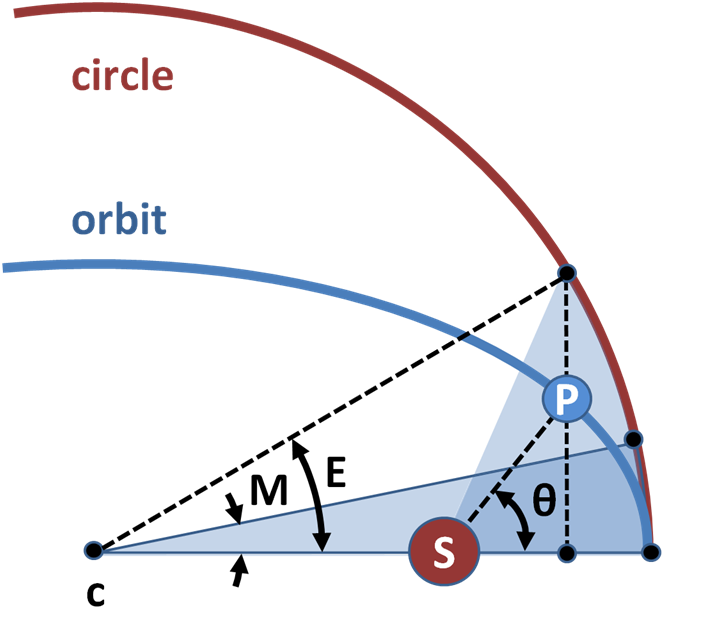
\includegraphics[scale=0.4]{Figures/Anomalies-MOD.png}
\caption[Diagram of Anomalies]{A diagram to compare the Eccentric, Mean and True anomalies of an orbiting planet.  The planet is marked as P, the central is S, and the center of the ellipse is C in this plot. }
\label{fig:Anomalies}
\end{center}
\end{figure}
%----------------------------------------------------------------------------------------------------------------------------------
\subsection{Converting between $T_o$ and $T_{ij}$}\label{sec:ToTcCalculator}

Used by the Radial Velocity model, not needed by the Astrometry model and is thus set to zero for those calculations.

In order to avoid biasing against circular solutions, one approach is to step through the parameter space using the Time of Inferior Conjunction ($T_{ij}$), instead of the Time of Periapsis ($T_o$).  From the Earth's prospective, $T_{ij}$ is when the companion object is located between the Earth and the primary (shown as {\color{green}$T_{ij}$} in Figure \ref{fig:ToTcDiagram}), and $T_o$ is when the companion crosses the plane of the sky moving away from the Earth, \citep{heintz}.  In the radial velocity method, at $T_{ij}$ the motion of the planet will be completely parallel to the plane of the sky, with no component along the line of sight to the Earth, resulting in a measured radial velocity of zero.  By understanding these two definitions, it is possible to calculate one from the other if the values for the eccentricity, {\it e}, and argument of periapsis, $\omega$, are known.

First, considering the plane of the sky is perpendicular to the line of sight (see Figures \ref{fig:orbElements} \& \ref{fig:ToTcDiagram}), it can be understood that the True Anomaly ($\theta_s$) of the companion at the Time of Inferior Conjunction will equal 90$^{\circ}$.  Then:

\begin{equation}\label{eq:one}
\theta_s = 90^{\circ}-\omega
\end{equation}

When the companion passes in front of the primary directly along the line-of-site, this location is referred to as the Time of Center Transit ($T_c$).  Although, in many cases the inclination of the system is not in the $90^{\circ}$+/-$10^{\circ}$ rough ranged needed, and no transit will be seen from Earth.

The Eccentric Anomaly of the companion can then be calculated from:

\begin{equation}
E_s = 2.0*\tan^{-1} \bigg( \sqrt{\frac{1.0-e}{1.0+e}} \frac{\sin(\frac{\theta_s}{2.0})}{\cos(\frac{\theta_s}{2.0})} \bigg)
\end{equation}
this equation is a manipulated version of that found in many texts, such as \citet{heintz}, seen below.

\begin{equation}
\tan\bigg( \frac{\theta_s}{2.0}  \bigg) = \sqrt{\frac{1.0+e}{1.0-e}} \tan\bigg( \frac{E_s}{2.0} \bigg)
\end{equation}

The Kepler's Equation, where $M_s$ is the Mean Anomaly of the secondary, (\citet{heintz} \& \citet{hilditch}), is given by:

\begin{equation}
M_s = E_s-e\times \sin(E_s)  
\end{equation}

Knowing the relations for the Mean Motion n:

\begin{subequations}
\begin{align}
n &= \frac{2\pi}{P}\\
n &=\frac{M_s}{t-T_o}=\frac{M_{ij}-M_{o}}{T_{ij}-T_o} 
\end{align}
\end{subequations}
where {\it t} is the epoch of observation and P is the orbital period.
We can then apply these to get the following equation assuming $M_{o}$ is zero.

\begin{equation}\label{eq:five}
\Delta t =t = \frac{M_{ij}P}{2\pi}
\end{equation}

%The value of $\Delta$t is forced to be inside one positive period by adding the period to it if (\ref{eq:5}) results in a negative value.

From this we can calculate either the Time of Inferior Conjunction, or Time of Periapsis knowing the other using:
\begin{subequations}
\begin{align}
T_{ij} &= T_{o}+\Delta t\\
T_o &= T_{ij}-\Delta t
\end{align}
\end{subequations}

%Extra non-necessary equations for my work, but I am writing them up for completion of the equations provided in the email.

%Finally a ratio of location in the orbit compared to periastron is calculated, this can also be thought of as a version of the orbital phase:
%\begin{equation}
%d_{min_s} = \frac{\Delta t}{P}
%\end{equation}

Knowing the primary object is just 180$^{\circ}$ out of phase with the companion, these equations can be used for the primary replacing $\theta_p$ for $\theta_s$ in Equation (\ref{eq:one}):
\begin{equation}
\theta_p = 90^{\circ}-\omega+180^{\circ}
\end{equation}


\begin{figure}[htp]
\begin{center}
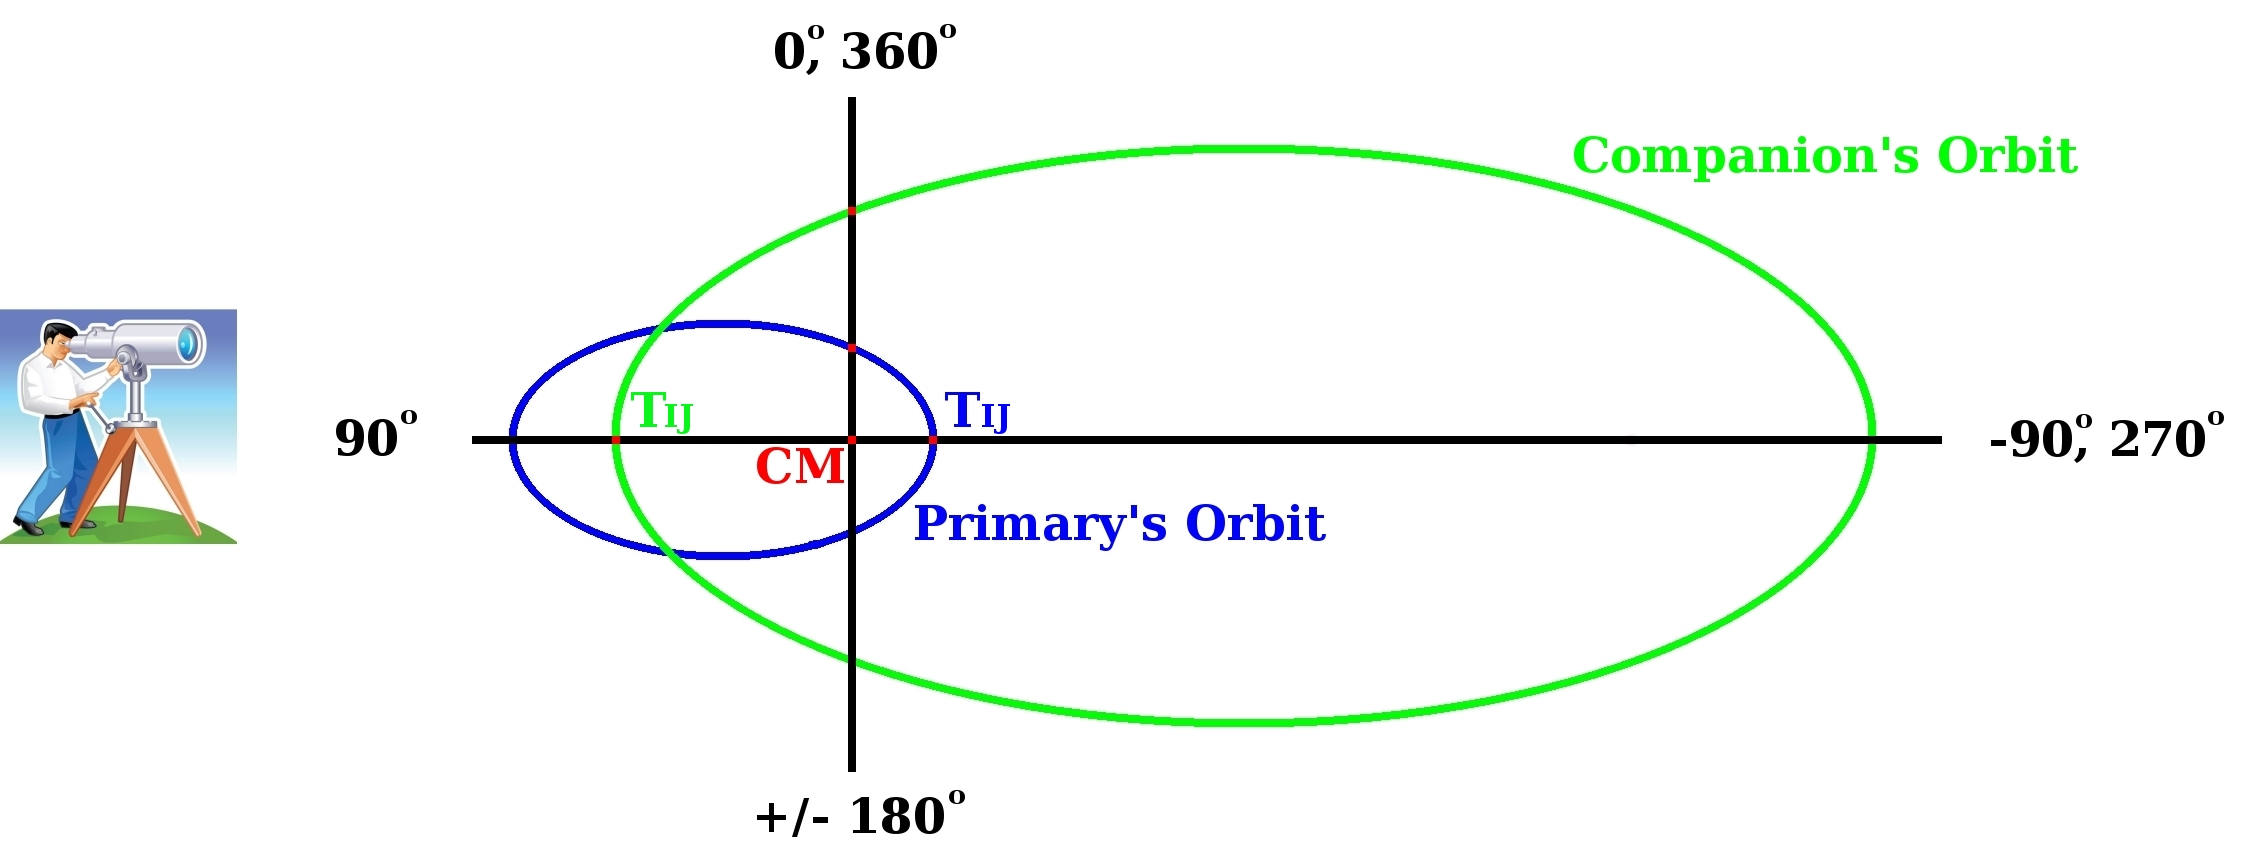
\includegraphics[scale=0.31]{Figures/TcToEllipses2-withTelescope4.jpeg}
\caption[Binary Inferior Conjunction Diagram]{A diagram showing the location of the Inferior Conjunction locations ({\color{green}$T_{ij}$} \& {\color{blue}$T_{ij}$}) of two objects in a binary system, orbiting the center of mass ({\color{red}CM}).}
\label{fig:ToTcDiagram}
\end{center}
\end{figure}

To take into account that $T_{ij}$ can occur before or after $T_{o}$ in a given system, the following conditionals are applied to get the correct value for $\Delta t$ produced by Equation (\ref{eq:five}):

\begin{equation}\label{eq:ToTcCorrections1a}
\Delta t = \left\{ \begin{array}{l l} \Delta t-P& \quad \text{ $\omega$ in [ 90$^{\circ}$,360$^{\circ}$], (T$_o$ $>$ T$_{ij}$)}\\  \Delta t& \quad \text{ $\omega$ in [-180$^{\circ}$,90$^{\circ}$], (T$_o$ $<$ T$_{ij}$)} \end{array} \right.
\end{equation}

these simplify to:
\begin{equation}\label{eq:ToTcCorrections1b}
\Delta t = \left\{ \begin{array}{l l} \Delta t-P& \quad \text{ $\omega$ $>$ 90$^{\circ}$, (T$_o$ $>$ T$_{ij}$)}\\  \Delta t& \quad \text{ otherwise, (T$_o$ $<$ T$_{ij}$)} \end{array} \right.
\end{equation}

When considering the values for the primary object (triggered with the `backhalf' boolean inside the function), these conditionals become:

\begin{equation}\label{eq:ToTcCorrections2a}
\Delta t = \left\{ \begin{array}{l l} \Delta t-P& \quad \text{ $\omega$ in [-180$^{\circ}$,270$^{\circ}$], (T$_o$ $>$ T$_{ij}$)}\\  \Delta t& \quad \text{ $\omega$ in [ 270$^{\circ}$,360$^{\circ}$], (T$_o$ $<$ T$_{ij}$)} \end{array} \right.
\end{equation}

simplifying to:
\begin{equation}\label{eq:ToTcCorrections2b}
\Delta t = \left\{ \begin{array}{l l} \Delta t-P& \quad \text{ $\omega$ $>$ 270$^{\circ}$, (T$_o$ $>$ T$_{ij}$)}\\  \Delta t& \quad \text{ otherwise, (T$_o$ $<$ T$_{ij}$)} \end{array} \right.
\end{equation}

Therefore, with these equations, one only needs to step through the parameter space along one of them and calculate the other from it, along with {\it e}, P and $\omega$.


%-------------------------------------------------------------------------------------------------------------
\subsection{Differences Between Investigating Stellar or Planetary Companion}\label{sec:omegaIssues}

NOTE: my recent investigations have found below to be essentially backwards!!! ie. put omega into DI and omega+180 into RV equations, using standard omega to calculate Tc !!!

The key difference when investigating a planetary compared to that of a stellar companion is the values of {\it a} and $\omega$ used in the astrometry model.  As discussed in \citet{Shulze-Hartung} and \citet{wright2009}, when the companion is a planet, the values of for the star are used, ie $a_1$ and $\omega_1$.  This is because the method was originally developed to find the orbit of the primary about the system's center of mass as the secondary was not seen.  More recently though, in most cases the companion is seen and the astrometric values are for the location of the secondary relative to the primary instead of the center of mass.  In these cases the apparent orbit is for the combined system and the values input into the astrometric model are $a_1+a_2$ and $\omega_2+\pi$, using the convention $\omega_1$ = $\omega_2+\pi$.

One must be careful to take this into account when doing 3D simulations, to ensure that $\omega_2+\pi$ is passed into the astrometry model and simply $\omega_2$ is used in the radial velocity one.

\pagebreak

%--------------------------------------------------------------------------------------------------------------------------------------

\subsection{Direct Imaging (Astrometry) Model: Using the Thiele-Innes Method}\label{sec:TH_I} 

The measurement of the astrometry values in the data, and the matching ones from the Thiele-Innes method applied here, are discussed in section \ref{sec:MeasAstrometry}.

The Thiele-Innes method to solve for the orbital elements of binary systems was first described in \citet{Thiele}, and later advanced with the inclusion of the Innes constants formulated in \citet{Van}.  This approach has been mainstream ever since, and the equations to find the ephemeris are given below can be found in many text books, such as \citet{aitken}, \citet{binnendijk} and \citet{heintz}.

\begin{subequations}
\begin{align}\label{eq:24a}
A& = a[\cos(\Omega)\cos(\omega)-\sin(\Omega)\sin(\omega)\cos(i)]\\
\label{eq:24b}
B& = a[\sin(\Omega)\cos(\omega)+\cos(\Omega)\sin(\omega)\cos(i)]\\
\label{eq:24c}
F& = a[-\cos(\Omega)\sin(\omega)-\sin(\Omega)\cos(\omega)\cos(i)]\\
\label{eq:24d}
G& = a[-\sin(\Omega)\sin(\omega)+\cos(\Omega)\cos(\omega)\cos(i)]
\end{align}
\end{subequations}

The x and y components of the location on the apparent ellipse are found with:
\begin{subequations}
\begin{align}\label{eq:28-1a}
x_{TH-I}& = AX+FY\\
\label{eq:28-1b}
y_{TH-I}& = BX + GY
\end{align}
\end{subequations}

knowing,

\begin{subequations}
\begin{align}\label{eq:28-1.5a}
X& = \frac{r_j}{a}\cos(\nu_j) =\cos(E_j)-e\\
\label{eq:28-1.5b}
Y& = \frac{r_j}{a}\sin(\nu_j) = \sqrt{1-e^2}\sin(E_j) 
\end{align}
\end{subequations}
where, $\nu$ is the True Anomaly, E is the Eccentric Anomaly and r is the distance between the object and the primary at a particular time in the orbit; if the value of a is the semi-major axis of the secondary alone, instead of the combined system, then the value for r is the distance between the secondary and the center of mass.  These are the only equations where the current position in the orbit is taken into account, and it is critical for making the predicted x, y values match the observed ones at a particular epoch (j).

%Equations (\ref{eq:4.1.1} - \ref{eq:4.1.5b}) are then used to calculate the epoch dependant values: the True Anomaly ($\theta$), Mean Anomaly (M), and Eccentric Anomaly (E).

As mentioned before, the respective x and y values can be calculated from the measured position angle ($\phi$) and separation angle ($\rho$), in the units of [rads] and [$\arcsec$] respectively, given:
\begin{subequations}
\begin{align}\label{eq:28-2a}
x_{TH-I}& = \rho \cos(\phi)\\
\label{eq:28-2b}
y_{TH-I}& = \rho \sin(\phi)
\end{align}
\end{subequations}
\pagebreak
%----------------------------------------------------------------------------------------------------------------------------------

\subsection{Radial Velocity Model}\label{sec:RV-OrbModels}

In the case of calculating the radial velocity residuals, there are various forms of the equation to calculate predicted radial velocity of the host star due to its companion's motion.

One very important thing that needs to be taken into account for radial velocity equations, that does not effect in direct imaging calculations, phase offset.  This is the phase difference between the location of the companion at closest approach and inferior conjunction; in cases where the inclination is $\sim$90, the companion passes in front of the primary and the inferior conjunction is also referred to as the location of center transit.  To take this into account, a manipulated version of the Mean Anomaly equation is used, which in turn effects the value of the True Anomaly used in the following radial velocity calculations.
%\subsubsection{Inputs}
\begin{table}[h]
\centering
\caption{ Inputs to the Radial Velocity Model.}
\begin{tabular}{c c c}
\hline\hline
Parameter & Description & Typical Range \\
\hline
t* & epoch of observation/image [julian date] & n/a\\
Sys$\_$Dist* & measured system distance from Earth [PC] &  [0.01,50.0]\\
{\it i} & inclination [$^{\circ}$] & [0,180]\\
$\omega$ & Argument of Periapsis [$^{\circ}$] & [0,360]\\
e & eccentricity of orbits [unitless] & [0.001,0.999]\\
T & Last Periapsis Epoch/time [julian date] & [t-period,t]\\
$T_c$* & Last Transit Center Epoch/time [julian date] & [t-period,t]\\
period & period of orbits [yrs] & [1.0,100.0]\\
a*** & Total Semi-major axis [AU]  & [0.1,200] \\
Mass1*** & Mass of primary star [M$_{\sun}$] & [0.001,10] \\
Mass2*** & Mass of companion [M$_{\sun}$] & [0.001, Mass1] \\
K*** & Semi-major Amplitude of primary star [m/s]& [1,500]\\
verbose & Send prints to screen? [True/False](Default = False) & n/a\\
\hline
\end{tabular}
\\
  * = Normally measured/known (ie. not random numbers).\\
 *** = Optional.
\end{table}

%\subsubsection{Outputs}

\begin{table}[h]
\centering
\caption{ Outputs of the Radial Velocity Model.}
\begin{tabular}{c c}
\hline\hline
Parameter & Description \\
\hline
vr & Radial Velocity of primary due to companion [m/s] \\
K & Semi-major Amplitude of primary star [m/s]\\
\hline
\end{tabular}
\end{table}

\pagebreak

Use the Mean Motion, n, time of current epoch (t), time of last periapsis (T), and time of transit center transit (Tc) to get the updated Mean Anomaly:
\begin{subequations}\label{eq:RV-Ma}
\begin{align}
phase& = \frac{Tc-T}{period_{days}} \\
%int\bigg(\frac{Tc-T}{period_{days}}\bigg)period_{days}
\label{eq:RV-Mb}
M& = n \bigg[ \frac{(t-T)}{365.25} +phase \bigg]\\
\end{align}
\end{subequations}
%where `int()' refers to taking the integer value of what is in the brackets.  
The phase of the companion in Equation (\ref{eq:RV-Ma}) is unit-less value between 0 and 1.  In Equation (\ref{eq:RV-Mb}), the first term is essentially a fraction of how far the current epoch is away from the time of last periapsis multiplied by the Mean Motion throughout the orbit, resulting in units of radians.  Following these equations (\ref{eq:4.1.3})-(\ref{eq:4.1.5b}) would be used to calculate the True Anomaly needed in the radial velocity calculations shown below.  This modified version of the Mean Anomaly equation is only needed when the eccentricity is non-zero, else Tc is set equal to {\it T} resulting in a zero phase, so this version reduces to the original form shown in (\ref{eq:4.1.2}).
%It was found that because of the sine function in (\ref{eq:4.1.4}), shifting the phase ahead into a positive value within $2\pi$ was the best .

The most common form of the radial velocity equation is:
\begin{equation}\label{eq:rvStandard}
vr =  K[\cos(\theta+\omega_2)+e \cos(\omega_2)]
\end{equation}
where {\it K} is the semi-major amplitude of the radial velocity curve.

The different formulations for calculating {\it K} are related to each other by Kepler's third law, given in Equation (\ref{eq:KepThird}).

To find the radial velocity of the primary star due to companion's orbital motion: %(version used in VRcalcStarStar:VRcalculator):
\begin{subequations}\label{eq:30}
\begin{align}\label{eq:K_general}
K_s &= \bigg[\frac{2\pi G}{P}\bigg]^{1/3}\frac{M_2}{M_1}(M_1+M_2)^{1/3}\frac{\sin(i)}{\sqrt{1-e^2}}\\
\label{eq:K_MassGeneral}
&=\bigg[\frac{2\pi G(M_1+M_2)}{P}\bigg]^{1/3}\frac{M_2}{M_1}\frac{\sin(i)}{\sqrt{1-e^2}} \\
\label{eq:K_semiMajor}
&= \frac{2\pi a_1\sin(i)}{P\sqrt{1-e^2}}
\end{align}
\end{subequations}

When the companion is a planet, it can commonly be assumed that Mass$_{planet} \ll$ Mass$_{star}$, so $M_1+M_2 \approx M_1$.  This simplifies the equation for {\it K} to:
\begin{equation}\label{eq:K_planetMass}
K_s = \bigg[\frac{2\pi G}{P}\bigg]^{1/3}\frac{M_2\sin(i)}{M_1^{2/3}}\frac{1}{\sqrt{1-e^2}}
\end{equation}

As the mass of each object is needed to calculate the semi-major axis of the primary, a$_1$, using  (\ref{eq:K_semiMajor}) keeps things simple making this the favored form.

Overall, this leads to 3 different ways to calculate the radial velocity of the primary due to a companion:

\begin{subequations}\label{eq:vr_finals}
\begin{align}\label{eq:vr_semiMajor}
vr_c \text{ or } vr_{p} &= \frac{2\pi a_1\sin(i)}{P\sqrt{1-e^2}}[\cos(\theta+\omega_2)+e \cos(\omega_2)]\\
\label{eq:vr_starMass}
vr_c&=\bigg[\frac{2\pi G(M_1+M_2)}{P}\bigg]^{1/3}\frac{M_2}{M_1}\frac{\sin(i)}{\sqrt{1-e^2}}[\cos(\theta+\omega_2)+e \cos(\omega_2)]\\
\label{eq:vr_planetMass}
vr_{p} &= \bigg[\frac{2\pi G}{P}\bigg]^{1/3}\frac{M_2\sin(i)}{M_1^{2/3}}\frac{1}{\sqrt{1-e^2}}[\cos(\theta+\omega_2)+e \cos(\omega_2)]
\end{align}
\end{subequations}

where $vr_c$ would be the radial velocity of the primary star due to a companion star, and $vr_p$ due to a companion planet around the same primary.  In the SMODT code, that of (\ref{eq:vr_semiMajor}) is referred to as ``vrCalculatorSemiMajorType", (\ref{eq:vr_starMass}) as ``vrCalculatorMassType", and (\ref{eq:vr_planetMass}) as ``vrCalculatorPlanetMassType", with the default in all cases being (\ref{eq:vr_semiMajor}).

%Velocity residual due to planet around primary star (version used in VRcalcStarPlanet: VRcalculatorsemi-majorType):
%\begin{equation}\label{eq:29}
%vr_p = \frac{2\pi a_1\sin(i)}{P\sqrt{1-e^2}}[\cos(\theta+\omega)+e \cos(\omega)]= K_p[\cos(\theta+\omega)+e \cos%(\omega)]
%\end{equation}

%Velocity residual due to planet around primary star (version used in VRcalcStarPlanet:VRcalculator):
%\begin{equation}\label{eq:31}
%vr_p = \bigg[\frac{2\pi G}{P}\bigg]^{1/3}\frac{M_2\sin(i)}{M_1^{2/3}}\frac{1}{\sqrt{1-e^2}}[\cos(\theta+\omega)+e \cos(\omega)] = K_p[\cos(\theta+\omega)+e \cos(\omega)]
%\end{equation}

%In \citet{Shulze-Hartung} an alternative formulation for the radial velocity equation is used that inputs the Eccentric Anomaly, E, instead of the True Anomaly, $\theta$.  The difference between these is is just a choice of parameters and they are both mathematically equivalent.

%Velocity residual due to companion star, or planet, used in \citet{Shulze-Hartung}:
%\begin{equation}\label{eq:32}
%vr = \frac{2\pi a_1 \sin(i)}{P(1-e\cos(E))}[\sin(E)\sin(\omega)-\sqrt{1-e^2}\cos(E)\cos(\omega)]
%\end{equation}

%\begin{subequations}\label{eq:32.2}
%\begin{align}
%vr_p& = \frac{2\pi a_1 \sin(i)}{P}\bigg [\frac{\sin(E)\sin(\omega)-\sqrt{1-e^2}\cos(E)\cos(\omega)}{(1-e\cos(E))}\bigg]\\
%& =\bigg[ \frac{2\pi G}{P}\bigg]^{1/3} \bigg[\frac{M_p \sin(i)}{(M_p+M_1)^{2/3}} \bigg] \bigg [\frac{\sin(E)\sin(\omega)-\sqrt{1-e^2}\cos(E)\cos(\omega)}{(1-e\cos(E))}\bigg]
%\end{align}
%\end{subequations}

%Although, whether $\omega$ is equal to $\omega_1$ or $\omega_2$ is not properly described in the paper.  Through personal communications with the author, it was clarified to be $\omega_2$ in all cases.  %Following their convention, we set $\omega_1 = \omega_2+\pi$, as it is arbitrary as long as it the convention is mentioned in any resulting research papers.

Finally the ${\chi}^{2} $ is calculated following:
\begin{equation}\label{eq:33}
{\chi}^{2} \equiv  \sum_{i=1}^{i=E} \frac{(model_i - observed_i)^{2}}{\sigma^{2}_i} = \sum_{i=1}^{i=E} \frac{[(vr_c+vr_p) - (RV_{data}-\gamma)]^{2}}{\sigma^{2}_i}
\end{equation}

where $\gamma $ is the velocity offset of that instrument.  In the case that the velocity of the system's center of mass WRT the Earth has not been removed, the observed component in (\ref{eq:33}) becomes ($RV_{data}-\gamma_{Instrument}-\gamma_{COM}$) (\citet{Paddock} \& \citet{Shulze-Hartung}).  When only investigating the radial velocity fit of a single companion, the other would naturally be zero in the above equation.

%----------------------------------------------------------------------------------------------------
\pagebreak
\bibliography{SMODT-citations}
\clearpage


\end{document}









